\section{Soft Tissue Simulation using Finite Elements}\label{methodology-fea}

\subsection{FEA concepts}

Finite element method (FEM) is a numerical method extremely useful in a wide variety of physical simulations. It finds applications in mechanical structural analysis, electrodynamics, hydraulics and many others. Such a wide range of applications arises from the fact that FEM can be used in approximately solving any \textit{field} problem \cite{Hutton2004}. A field problem, also known as a \textit{boundary value} problem, is a mathematical problem in which a set of dependent variables must satisfy a differential equation everywhere in the specified domain and satisfy the boundary conditions. \textit{Boundary conditions} are the predefined set of values that are applied to the boundary of the analyzed domain.

The main focus of this research is on mechanical structural analysis and particular in soft tissue simulation. \cite{Oden:2010} identifies two key attributes of FEM:

\begin{description}

  \item[Partitioning] \hfill \\
  The analyzed domain is partitioned into a set of small non-overlapping domains over which complex function can approximated by local polynomial function.

  \item[Weak-formulation] \hfill \\
  The local functions are not required to satisfy the analytical solution locally, as long as the overall domain integral satisfies the boundary conditions.

\end{description}

The finite sub-domains are also known as \textit{elements}. The subdivision principle is illustrated in Figure \ref{fea-fea}. For a detailed introduction to FEM refer to \cite{Hutton2004}.

\begin{figure}
\begin{center}
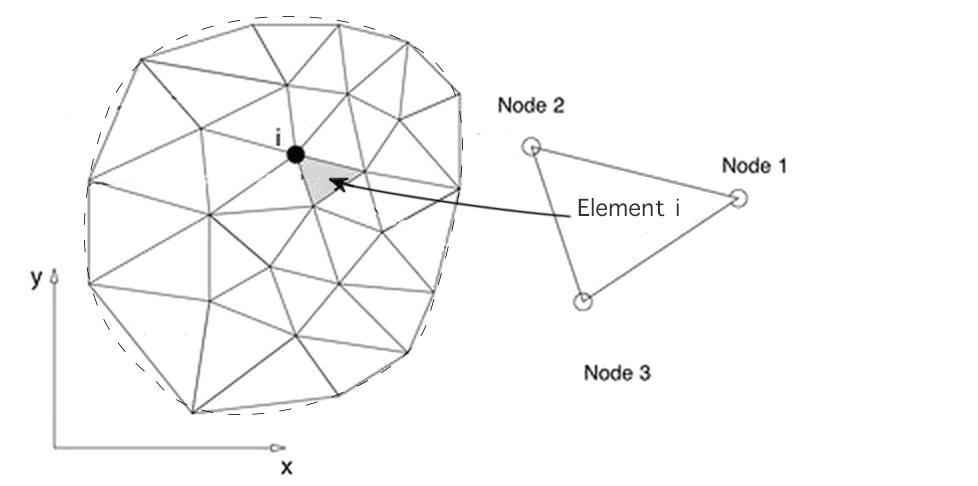
\includegraphics[width=100mm]{sections/methodology/images/fea/fea.png}
\caption[Finite element partitioning.]{\label{fea-fea}}
\end{center}
\end{figure}

In the case of surgical simulations FE model needs to predict the deformation \textit{field} within a particular organ that the surgery is aimed at. The \textit{boundary conditions} are the attachment tissues that connect and fix the organ to the body. The \textit{external loads} are the forces and deformations that are applied from the virtual surgical tools when they are in contact with the organ. The governing equation that the method is aimed to solve is:

\begin{equation}
\label{eq-governing}
\textrm{M} \ddot{U} + \textrm{D}\dot{U} + K(U)U = \textrm{R}
\end{equation}

where $M$ is the mass matrix, $U$ are the deformations of the FE nodes, $D$ is the damping matrix, $R$ are the externally applied loads. The $K(U)$ component is a stiffness matrix represented by a function of the deformations.

\subsection{Total lagrangian explicit dynamic FE}

  Total lagrangian explicit dynamic (TLED) is a variation on the Lagrangian formulations of FEM. It is initially proposed by \cite{Miller2007} as a means for efficient computer based finite element analysis. The alternative approach is known as the Updated lagrangian explicit dynamic approach is based on using the previously calculated configuration of the deformed body in order to calculate the stresses occurring in the finite elements. In contrast to this technique TLED uses the original reference configuration to perform the calculations. TLED has the advantage of allowing precomputations of a large chunk of data as compared to the approach using the updated lagrangian.

  TLED is a very efficient explicit FEA algorithm that is very useful in surgical simulations. The details of the algorithm and the derivation of the formulation are presented in paper \cite{Miller2007}

\paragraph{Discussion} The TLED scheme provides very accurate and efficient simulations for soft-tissue simulation. However, as the authors described it, it is more suitable for simulating ``very soft'' tissues. In cases when the stiffness of the material is higher the minimal time-stem decreases exponentially leading to dramatically decreased simulation rates.

This makes it impossible to use the approach for simulating bony structures present in childbirth. The fetal head and maternal pelvis deformations cannot be performed using TLED approach. Additionally, it is possible that certain tissues in the pelvic floor may have sufficiently high Young's moduli making it impractical to simulate them using TLED.

\subsubsection{Basic algorithm} \label{fea-algorithm}

The algorithm can be divided into 3 distinct steps:

\begin{enumerate}

  \item Precomputation
  \item Initialization
  \item Time stepping

\end{enumerate}

Note how the precomputation step is a separate entry which allows excluding the computational effort from the main update loop. The reason why the values can be precomputed becomes clear when the notation used in \cite{bathe:1996} is applied. The $0$ on left size of the symbols indicate that the value is for the initial reference configuration which stay constant throughout the simulation.

Here we provide a more detailed break-down of the steps:

\begin{enumerate}

  \item Preprocessing

  \begin{enumerate}

    \item Read the input file and load the mesh along with other assembly information (constraints, external loads, etc).
    \item For each element of the mesh compute the following quantities

    \begin{itemize}

      \item Jacobian determinant $det(\textbf{J})$
      \item Spatial derivatives of the shape functions $\partial{\textbf{h}}$
      \item Strain-displacement matrices $_{0}^{t}\textrm{\textbf{B}}_{L0}$
    \end{itemize}

    \item Compute the diagonalized (lumped) mass matrix $^{0}M$ representing the mass of the whole mesh

  \end{enumerate}

  \item Initialization \label{fea-algorithm-initialization}
  \begin{itemize}
    \item Set the nodal displacements $\textbf{u}$ to the prescribed values and add prescribed external force loads into $\textbf{R}$
  \end{itemize}

  \item Time-stepping
  \begin{itemize}
    \item For each element:
    \begin{enumerate}
      \item Compute deformation gradient $_{0}^{t}\textrm{\textbf{X}}$ based on the previous nodal deformations
      \item Compute the strain-displacement matrix for the current configuration using the transpose of  the new deformation gradient $_{0}^{t}\textrm{\textbf{X}}$ and the precomputed strain-displacement for the reference configuration $_{0}^{t}\textrm{\textbf{B}}_{L0}$:
        \begin{equation}
        \label{eq-stress-strain}
        _{0}^{t}\textrm{\textbf{B}}_{L}^{(k)} = _{0}^{t}{\textrm{\textbf{B}}_{L0}^{(k)}}
        _{0}^{t}\textrm{\textbf{X}}^{T}
        \end{equation}


      \item Compute the Second Piola-Kirchoff stress $_{0}^{t}\textrm{\textbf{S}}$ according to:
        \begin{equation}
        \label{eq-spk}
        _{0}^{t}\textrm{\textbf{S}} =
          det(_{0}^{t}\textrm{\textbf{X}})
            _{t}^{0}\textrm{\textbf{X}}^{t} \tau _{t}^{0}\textrm{\textbf{X}}^{T}
        \end{equation}

      \item Compute reaction forces for the nodes of the current element. An efficient way of evaluating the integral in the equation is using a Gaussian quadrature.

      \begin{equation}
      \label{eq-reaction-forces}
      ^{t}\textrm{F}^{(m)} =
      \int_{0_{V}}{_{0}^{t}\textrm{\textbf{B}}_{L}^{T}
        \textrm{ }
        _{0}^{t}\textrm{\textbf{S}}
        \textrm{ }
        d^{0}V}
      \end{equation}
    \end{enumerate}

    \item For each node:

    \begin{enumerate}

      \item Update the deformation of the current node using a time-integration method (e.g. Central Difference Method)

      \item \label{fea-algorithm-external-loads} Apply the imposed values to nodal displacements $\textbf{u}$ and add current external force loads into $\textbf{R}$

    \end{enumerate}

  \end{itemize}

\end{enumerate}


\subsection{CPU based implementation}

  Our CPU based implementation of the algorithm is essentially a direct translation of the above algorithm into C++. By using appropriate data-structures and custom built matrix routines we were able to achieve basic TLED functionality.

  \subsubsection{Data-structures}

  Figure \ref{fea-cpu-data-structures} gives a basic overview of the data-structure framework used in our TLED implementation.


  \begin{figure}
  \begin{center}
  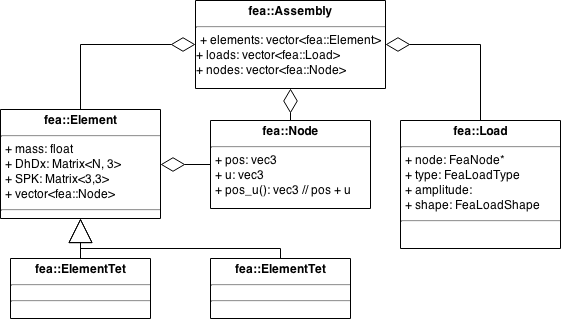
\includegraphics[width=120mm]{sections/methodology/images/fea/cpu-data-structures.png}
  \caption[Basic overview of TLED implementation in BirthView.]{\label{fea-cpu-data-structures}}
  \end{center}
  \end{figure}



  \subsubsection{Traditional FEA simulation}

  Traditionally FE analyses are performed on a particular setup with fixed parameters. Time frame is one the most important aspects of the simulation. To perform an analysis a starting time and a finishing time are normally chosen and the simulation is commenced. The natural and essential external loads are varied throughout the timeframe according to well defined laws and functions. This kind of simulations are done in the modern FEM packages like Dassault Systems Abaqus or Siemens

  The developed BrithView TLED simulation system is capable of performing this type of a simulation. The dedicated component class called \textit{FixedTimeSimulationComponent} can be used to perform a fixed-time simulation.

  The advantage of such type of simulations is apparent when a highly controlled analysis environment is required. When testing the stability and strength of mechanical structures such simulations allow greater control and repeatability of the analyses.

  However, there are cases when the analysis is required to flow continuously throughout the simulation. For such cases we have developed an alternative simulation framework described in section \ref{methodology-fea-interactive}.

  \subsubsection{Interactive real-time simulation}\label{methodology-fea-interactive}

  The typical scenario of a training session will involve user input. Due to the lack of control over what the input is, various aspects of the simulation remain completely unpredictable. User input can be erroneous and unexpected, especially in the case of a novice trainee. The non-interactivity makes the traditional simulations unusable in cases of real-time training sessions.

  In contrast to the previously described type of FE simulation, an interactive simulation is not limited to a fixed timeframe. The simulation is run continuously throughout the training session and the  input from the user is continuously transformed into external loads acting on the assembly.


  \subsubsection{Experiments}

  A simple test scene was created where a single soft cube is stretch in the positive $x$ axis by an essential load. An essential load is applied directly onto the nodes as a displacement, without involving integrating forces.

  Figure \ref{fea-cube-old} shows the experimental results reported in \cite{Miller2007}. A simple 1000 element (10 by 10 by 10) cube is fixed on one side. The opposite side is stretched by 30\% of cube's dimension along the direction of the stretch. We replicated the identical experiment so to simplify validation by having identical models.
  % !!!!!!!!!!!!!!!!!!!!!!!!!

  \begin{figure}
  \begin{minipage}[t]{6cm}
  \begin{center}
  \includegraphics[width=65mm]{sections/methodology/images/fea/cube-tled-original.png}
  \caption[A soft cube undergoing uniaxial stretch in \cite{Miller2007}]{\label{fea-cube-old}}
  \end{center}
  \end{minipage}
  \hfill
  \begin{minipage}[t]{6cm}
  \begin{center}
  \includegraphics[width=65mm]{sections/methodology/images/fea/cube-tled-new.png}
  \caption[Results from our implementation of TLED analysis on the same cube.]{\label{fea-cube-new}}
  \end{center}
  \end{minipage}
  \end{figure}

  More detailed benchmarking and validation is required to be done in the future.
